\documentclass[a4paper, 12pt]{report}

% Packages
\usepackage{xargs}
\usepackage[pdftex,dvipsnames,table]{xcolor}
\usepackage{tocloft}
\usepackage[utf8]{inputenc}
\usepackage[T1]{fontenc}
\usepackage[british,francais]{babel}
\usepackage{lmodern}
\usepackage{graphicx}
\usepackage{float}
\usepackage[pdfpagelabels,%
            urlbordercolor={.909803921569 .796078431373 .552941176471},%
            linkbordercolor={.839215686275 .4862745098 .482352941176},%
            citebordercolor={.839215686275 .607843137255 .447058823529},%
            pdftex,%
            pdfauthor={Alban Chazot},%
            pdftitle={Détection et classification d'objets dans un flux vidéo sphérique},%
            pdfsubject={Rapport de stage de 5A STI},%
            pdfkeywords={réseaux neuronaux, apprentissage profond, traitement de l'image, reconnaissance d'objets, temps réel},%
            pdfproducer={pdfTeX 3.14159265-2.6-1.40.15 (TeX Live 2015/dev/Debian)},%
            pdfcreator={Atom 1.14.3},%
            ]{hyperref}
\usepackage{cleveref}
\usepackage[nonumberlist]{glossaries}
\usepackage{svg}
\usepackage{parskip}
\usepackage{url}
\usepackage{amsmath}
\usepackage{fancyhdr}
\usepackage{vmargin}
\usepackage{sectsty}
\usepackage{listings}
\usepackage{pdfpages}
\usepackage{titling}
\usepackage{lipsum}
\usepackage{microtype}
\usepackage{tabularx}
\usepackage{enumitem}
\usepackage{eurosym}
\usepackage[super]{natbib}
\usepackage[colorinlistoftodos,prependcaption,textsize=tiny]{todonotes}
\usepackage{booktabs} %for rules
\usepackage{multirow}

% Macros
\definecolor{siisky}{HTML}{7AAEDD}
\definecolor{siiblue}{HTML}{0061AA}
\definecolor{siiorange}{HTML}{D64911}
\definecolor{siiorange2}{HTML}{FA6900}
\definecolor{siigrey}{HTML}{333D41}
\definecolor{siigrey2}{HTML}{667074}
\definecolor{siigreen}{HTML}{334100}
\definecolor{siigreen2}{HTML}{667400}
\definecolor{siipurple}{HTML}{8D338A}
\definecolor{siipurple2}{HTML}{C066BD}
\newcommandx{\content}[2][1=]{\todo[linecolor=red,backgroundcolor=red!25,bordercolor=red,#1]{#2}}
\newcommandx{\change}[2][1=]{\todo[linecolor=blue,backgroundcolor=blue!25,bordercolor=blue,#1]{#2}}
\newcommandx{\info}[2][1=]{\todo[linecolor=OliveGreen,backgroundcolor=OliveGreen!25,bordercolor=OliveGreen,#1]{#2}}
\newcommandx{\improvement}[2][1=]{\todo[linecolor=Plum,backgroundcolor=Plum!25,bordercolor=Plum,#1]{#2}}
\newcounter{descriptcount}
\renewcommand{\arraystretch}{1.5}
\newcolumntype{b}{X}
\newcolumntype{s}{>{\hsize=.5\hsize}X}
\newcolumntype{r}{>{\hsize=.2\hsize}X}
\newcolumntype{P}{>{\centering\hsize=.125\hsize}X}
\newcolumntype{Y}{>{\centering\arraybackslash}X}
\newcommand{\keywords}[1]{\par\textbf{Mot clefs:}\par\quad #1}
\newcommand{\blankpage}{\leavevmode\thispagestyle{empty}\setcounter{page}{0}\newpage}
\newcommand{\nocounter}{\thispagestyle{empty}\setcounter{page}{0}\pagebreak}
\newcommand{\todoref}{\textcolor{red}{\textbf{[REF]}}}
\newcommand{\specialcell}[2][c]{\begin{tabular}[#1]{@{}c@{}}#2\end{tabular}}

% Document info
\title{Détection et classification d'objets dans un flux vidéo sphérique}
\author{Alban Chazot}
\date{\today}

% Header + footer
\makeatletter
\let\thetitle\@title
\let\theauthor\@author
\let\thedate\@date
\makeatother

% Pages setup
\pagestyle{fancy}
\fancyhf{}
\rhead{\theauthor}
\lhead{\thetitle}
\cfoot{\thepage}
\setmarginsrb{3 cm}{2.5 cm}{3 cm}{2.5 cm}{1 cm}{1.5 cm}{1 cm}{1.5 cm}
\setlength{\parindent}{15pt}
\setcitestyle{super,open={},close={}}
\setlist{nolistsep}
\setlength{\aboverulesep}{0pt}
\setlength{\belowrulesep}{0pt}
\setlength{\extrarowheight}{.0ex}
%\linespread{1.05}

% Glossary
% Magic here
\makeglossaries

\newglossaryentry{lidar}
{
	name={LIDAR},
	description={\emph{LIght Detection And Ranging}, une technique de télémétrie (détermination de la distance d'un objet) qui se base sur la mesure du temps écoulé entre l'émission et la réception d'un faisceau de lumière. Dans notre cas, la source de lumière est un laser émettant de l'infrarouge. Par extension, on nomme LIDAR le dispositif matériel permettant de telles mesures}
}

\newglossaryentry{slam}
{
	name={SLAM},
	description={\emph{Simultaneous Localization And Mapping}, technique qui consiste, pour un robot ou véhicule autonome, à simultanément construire ou améliorer une carte de son environnement et de s’y localiser}
}

\newglossaryentry{gpu}
{
	name={GPU},
	description={\emph{Graphic Processing Unit}, Processeur possédant une structure hautement parallèle, permettant des calculs matriciels beaucoup plus rapides qu'avec un processeur possédant une architecture plus classique (CPU) et de ce fait utilisé principalement pour les traitements graphiques tels que le rendu 3D}
}

\newglossaryentry{poc}
{
	name={POC},
	description={\content{à développer}\emph{Proof Of Concept}}
}

\newglossaryentry{bu}
{
	name={BU},
	description={\emph{Business Unit}, unité organisationnelle au sein du groupe SII s'adressant à un secteur d'activité particulier}
}

\newglossaryentry{b2b}
{
	name={B2B},
	description={\emph{Business to Business}, caractérise les activités d'une entreprise visant une clientèle d'entreprises}
}

\newglossaryentry{rd}
{
	name={R\&D},
	description={\emph{Recherche et Developpement}, caractérise les activités d'une entreprise visant à accroître ses connaissances au travers de la recherche fondamentale et appliquée et à effectuer des réalisations expérimentales de manière à créer des produits ou stratégies innovants}
}

\newglossaryentry{robo}
{
	name={SRT2M},
	description={\emph{Système Robotique tactique Multi-Mission}, nom du produit final porté par le projet dont il est question dans ce rapport, et par extension le démonstrateur lui-même}
}



% Contents
\begin{document}
{
	% Front page
	\hypersetup{pageanchor=false}
	\nocounter
	\includepdf[pages={-},offset=30mm -25mm]{premade/frontpage.pdf}
	\nocounter
	\blankpage
	\nocounter
	
	% Abstract
	\begin{otherlanguage}{british}
	\begin{abstract}
		This paper presents the outcome of my internship at SII in the context of my last year of formation in Information Technology Security provided by the institute INSA Centre Val de Loire. This internship falls in line with previous works promoting robotics within the Research \& Development department of the SII Bourges agency. In this context of rapid development of artificial intelligence, we propose a robotic system capable of simultaneously mapping its environment and detecting surrounding objects of interest. This system, called \gls{robo}, is dedicated to perform recognition missions in dangerous environments, 
		\par
		
		\keywords{réseaux neuronaux, apprentissage profond, traitement de l'image, reconnaissance d'objets, temps réel}
	\end{abstract}
\end{otherlanguage}

	\nocounter

	% Thanks
	\section*{Remerciements}
\phantomsection
{
	En prélude à ce rapport, j'aimerais exprimer mes remerciements chaleureux à M. Adel Hafiane, Professeur et Responsable du Laboratoire de Vision par Ordinateurs à l'INSA Centre Val de Loire et Docteur à l'Université du Missouri. J'aimerais particulièrement saluer son implication dans ce projet, tant pour son aide quand à la réalisation du projet que pour sa présence régulière malgrés de nombreux impératifs.
	\par
	Je souhaite remercier M. David Daumand, mon tuteur de stage, Ingénieur Logiciel chez SII, pour avoir su piloter ce projet et y avoir porté une importance telle qu'il puisse être mis en lumière devant des acteurs importants internes et externes à la société. J'aimerais souligner sa volonté de suivre notre équipe de près en dépit du peu de temps dont il disposait.
	\par
	Merci à M. Fabrice Bosch, Directeur de l'agence SII Bourges, pour nous avoir fait confiance quand au choix du matériel à acquérir et pour ses encouragements au long du développement du projet.
	\par
	Finalement, merci à toute l'équipe de l'agence SII Bourges pour leur accueil chaleureux, l'ambiance conviviale des locaux et tous les bons moments passés ensemble.
}

	\nocounter

	% TOC
	\setlength{\cftbeforetoctitleskip}{-7.9em}
	{\footnotesize \tableofcontents}
	\nocounter

	% Introduction
	\hypersetup{pageanchor=true}
	\setcounter{page}{1}
	\section*{Introduction}
\phantomsection
\addcontentsline{toc}{section}{Introduction}
	
	% Contexte
	Ce document relate le travail qui a été effectué au sein du pôle recherche et développement de l'agence de SII Bourges, dans le cadre d'un stage de fin d'études à l'issue de la formation en Sécurité et Technologies Informatique de l'INSA Centre Val de Loire, option Architecture et Sécurité Logicielle.
	
	% Place du projet dans l'entreprise
	La mission s'inscrit dans la continuité du projet robotique du pôle R\&D en coopération avec l'INSA Centre Val de Loire, dont un précédant stage en avait fait l'objet. Cependant, il convient de préciser que le produit présenté ne se base pas sur le précédent travail, si ce n'est dans l'esprit de sa réalisation et de ses objectifs à long terme. En effet, il a pour vocation de faire croître le savoir-faire du pôle face aux problématiques appliquées du traitement du signal et de mettre en avant ces compétences devant des acteurs clés.
	
	% Description du projet
	Le projet est une preuve de concept, dont la finalité répond à la dénomination \emph{Système Robotique Tactique Multi-Missions pour la Surveillance et l'Aide à la Prise de Décision en Milieux à Risques} (SRT2M). Le système opérationnel final permet de recueillir des informations stratégiques sur l'environnement où il sera déployé, sans mettre en danger des acteurs humains. Ce \gls{poc} a fait l'objet de deux stages dont les sujets sont étroitements liés. Le premier, qui vise à effectuer une cartographie des lieux grâce à un \gls{lidar}, ne sera pas détaillé dans ce rapport. La mission décrite ici consiste principalement à concevoir et implémenter un système de détection et classification d'objets d'intérêt dans un flux vidéo sphérique, ainsi qu'une brique logicielle servant d'interface à la visualisation de ce flux vidéo agrémenté des résultats de la détection.
	
	% Présentation du plan
	Le plan.

		
	% Chapters
	\chapter{Présentation du contexte}
{
	\section{La Société pour l'Informatique Industrielle}
	{
		\subsection{Acteur de la transformation numérique}
		{
			\par
			{
				SII, ou Société pour l'Informatique Industrielle, est une entreprise de services du numérique implantée dans dix-huit pays (voir \autoref{fig:sii_impl}) au travers de soixante-six agences. Elle propose de multiples services en \gls{b2b}, dont principalement l'étude et le conseil en technologies sur la maîtrise d'ouvrage de projets et la conception et l'intégration de systèmes.
			}
			
			\begin{figure}[h]
			{
				\centering
				\includegraphics[page=1,width=0.92\textwidth]{figures/sii_impl.pdf}
				\caption{Implantation de SII au travers du monde\cite{sii_rf}}
				\label{fig:sii_impl}
			}
			\end{figure}
			
			\par
			{
				\content{TODO: continuer}
				L'activité au sein de l'entreprise s'organise en unités organisationnelles (\emph{Business Units}, ou \gls{bu})
			}
			
			\par
			{
				La fiche signalétique suivante donne une vue d'ensemble de l'entreprise, ainsi qu'elle permet de donner un contexte de réalisation du stage:
			
				\begin{description}
					\item[Nom de l'entreprise:] Société pour l'informatique industrielle (SII)
					\item[Date de création:] 1979\cite{sii_rf}
					\item[Statut juridique:] Société anonyme à directoire et conseil de surveillance
					\item[Siège social:] Paris
					\item[Effectif:] 5949\cite{sii_rs_2017}
					\item[Chiffre d'affaire:] 438,85M\euro\cite{sii_rs_2017}
					\item[Capital:] 103M\euro\cite{sii_rf}
					\item[Direction:] Patrice Demay (directeur général France), Eric Matteucci (président du directoire) et Jean-Paul Chevée (directeur général international)
					\item[Secteurs d'activité:] Aérospatiale, Banque, Défense, Énergie, Finance, Industrie, Média, Télécoms, Transports
					\item[Site internet:] \url{http://www.groupe-sii.com}
				\end{description}
			}
			
			% \begin{figure}
			% 	\centering
			% 	\begin{minipage}{.5\textwidth}
			% 		\centering
			% 		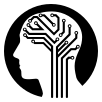
\includegraphics[page=1,width=0.7\linewidth]{figures/test.pdf}
			% 		\captionof{figure}{Test left}
			% 		\label{fig:Test2}
			% 	\end{minipage}%
			% 	\begin{minipage}{.5\textwidth}
			% 		\centering
			% 		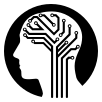
\includegraphics[page=1,width=0.7\linewidth]{figures/test.pdf}
			% 		\captionof{figure}{Test right}
			% 		\label{fig:Test3}
			% 	\end{minipage}
			% \end{figure}
		}
		\subsection{Historique}
			
			\par
			{
				\change{Trouver une meilleure phrase}
				Quelques dates clefs de l'évolution de l'entreprise:
			}
			
			\begin{description}
			{
				\item[1979:] Création de l'entreprise à Paris par Bernard Huvé, alors ingénieur consultant.
				\item[1984:] À l'occasion d'un contrat avec le laboratoire d'IBM, une deuxième agence est ouverte à nice.
				\item[1987-1989:] Déploiement de SII en Île-de-France avec la création des deux agences de Cergy Pontoise et Vélizy.
				\item[1992:] À la suite d'évolutions importantes du secteur de l'informatique, l'entreprise se recentre sur l'assistance technique et obtient la certification ISO 9001.
				\item[1997:] Ouverture des agences de Rennes et Aix-en-Provence.
				\item[1999:] Introduction en bourse de l'entreprise.
				\item[2000-2007:] Accroissement du maillage national: ouverture d'agences à Bordeaux, Brest, Caen, La Ciotat, Lannion, Le Mans, Lyon, Niort, Montpellier, Tours et Vitrolles. Ouverture de filiales internationales en République Tchèque et en Pologne.
				\item[2010:] Acquisition de AIDA Development, société allemande, qui permet à l'entreprise de pénétrer le premier marché européen.
				\item[Août 2010:] Création de l'agence SII Bourges.
				\item[2015:] Implantation aux Pays-Bas et en Colombie.
				\item[2016:] Implantation aux Canada et en Angleterre.
			}
			\end{description}
			\improvement[inline]{Plus de détails ?}
	}
	\section{Développement et exposition du savoir-faire}
	
		\subsection{SII Research et le pôle robotique}
			
			\par
			{
				L'entreprise SII dispose d'un pôle innovation, incarné par le laboratoire \emph{SII Research}, qui vise à regrouper et structurer les projets relatifs à l'innovation technologique. Contrairement au fonctionnement des \gls{bu}, elle ne s'addresse pas à un secteur d'activité ou un client particulier, mais vise à développer les connaissances et le savoir-faire du groupe en effectuant des activités telles que de la veille technologique, la gestion de la propriété intellectuelle et la gestion de projets \gls{rd} interne. A l'occasion de la réalisation de ces derniers, les acteurs du pôle sont amenés à réaliser des \gls{poc}, activité dans laquelle s'inscrit le projet \gls{robo}. Parmi leurs projets achevés, on peut citer \emph{CATED}, une application d'aide à l'autonomisation pour personnes autistes, \emph{Entrepôt Augmenté}, un projet utilisant la réalité augmentée pour optimiser le temps de traitement des commandes et \emph{TryAplane}, un système d'aide à la formation aéronautique.
			}
			\par
			{
				
			}
			
		\subsection{Technologies de pointe}
		
			\content[inline]{A faire}
			
}

	\chapter{Donec auctor}
	\section{Ligula dignissim}
		\subsection{Ornare eros}
			\lipsum[18-20]
		\subsection{Vivamus elit}
			\lipsum[21-22]
	\section{Morbi vel luctus}
		\subsection{Tellus tempor}
			\lipsum[23-24]
		\subsection{Pharetra}
			\lipsum[25-26]
	\section{Fermentum}
		\subsection{Varius at nunc}
			\lipsum[27-29]
		\subsection{Malesuada viverra}
			\lipsum[30-32]

	\chapter{Conception et développement}

	\section{Architecture du logiciel}

		\subsection{Vision globale}
			
			\content[inline]{A faire}

		\subsection{Traitement de données}

			\content[inline]{A faire}
			
		\subsection{Interface Homme-Machine}
		
			\content[inline]{A faire}

	\section{Détails de traitements}
	
		\subsection{Transmission de la vidéo}
		
			\content[inline]{A faire}
			
		\subsection{Transformation vidéo}
		
			\content[inline]{A faire}
			
		\subsection{Présentation vidéo et incrustation}
		
			\content[inline]{A faire}
			
	\section{Méthodes de travail}

		\subsection{Git-flow}
		
			\content[inline]{A faire}
			
		\subsection{Emprunts agiles}
		
			\content[inline]{A faire}
			

	\section{Pérennisation du projet}
	
		\subsection{Manuel utilisateur}
		
			\content[inline]{A faire}
			
		\subsection{Documentation}
		
			\content[inline]{A faire}
			
		\subsection{Installation automatique}
		
			\content[inline]{A faire}
				

	\chapter{Bilan et retour d'expérience}

	\section{Qualité des résultats}
	
		\content[inline]{A faire}

	\section{Perspectives d'évolution}
	
		\content[inline]{A faire}

	\section{Impact du projet}
		
		->nexter robotics
		\content[inline]{A faire}
	
	\section{Bilan personnel}
	
		\content[inline]{A faire}

	
	% Glossary
	\setglossarystyle{altlist}
	\printglossary[title={Glossaire}, toctitle={Glossaire}]
	\newpage
	\listoffigures
	
	% Bibliography
	\begin{thebibliography}{9}

	\bibitem{sii_rf}
		Groupe SII,
		\emph{Document de référence 2015/2016},
		04/08/2016,
		\par
		\url{http://www.groupe-sii.com/pfw_files/cma/regulatory_information/SII_DF_DREF_2015_2016_FR.pdf}
	
	\bibitem{sii_rs_2017}
		Groupe SII,
		\emph{Comptes annuels 2016/2017},
		06/06/2017,
		\par
		\url{http://www.groupe-sii.com/pfw_files/cma/regulatory_information/SII_AF_RS_EX_2016_2017_FR.pdf}
	
	\bibitem{qr3d}
		Quentin Ménard,
		\emph{Reconstruction d’un environnement en 3D à partir d’images / d’un flux vidéo},
		2016
	
	\bibitem{dlmed}
		P. Mamoshina,A. Vieira, E. Putin, A. Zhavoronkov,
		\emph{Applications of Deep Learning in Biomedicine}
		Mai 2016,
		\url{https://www.ncbi.nlm.nih.gov/pubmed/27007977}

	\bibitem{dltra}
		Kyunghyun Cho, Bart van Merrienboer, Dzmitry Bahdanau,
		\emph{On the Properties of Neural Machine Translation: Encoder–Decoder Approaches}
		Octobre 2014,
		\url{https://arxiv.org/pdf/1409.1259v2.pdf}

	\bibitem{dlrec}
		William Song, Jim Cai,
		\emph{End-to-End Deep Neural Network for Automatic Speech Recognition}
		Juin 2015,
		\url{https://cs224d.stanford.edu/reports/SongWilliam.pdf}

	\bibitem{dlaut}
		Jen-Hsun Huang,
		\emph{Accelerating the race to self-driving cars}
		Janvier 2016,
		\url{https://www.ncbi.nlm.nih.gov/pubmed/27007977}
		
	
	\bibitem{viola}
		Paul Vioal et Michael J. Jones,
		\emph{Robust Real-time Object Detection},
		\par
		\url{www.hpl.hp.com/techreports/Compaq-DEC/CRL-2001-1.pdf}
	
	\bibitem{svm}
		Thorsten Joachims,
		\emph{SVMlight}
		14/08/2008
		\par
		\url{http://svmlight.joachims.org}
	
	\bibitem{hog}
		S. Belongie, J. Malik et J. Puzicha,
		\emph{Matching Shapes},
		ICCV,
		2001

	\bibitem{sift}
		David G. Lowe,
		\emph{Object recognition from local scale-invariant features},
		ICCV,
		1999,
		\url{http://www.cs.ubc.ca/~lowe/papers/iccv99.pdf}

	\bibitem{surf}
		Herbert Bay, Andreas Ess, Tinne Tuytelaars, Luc Van Gool,
		\emph{SURF: Speeded Up Robust Features},
		CVIU 110,
		2008,
		\url{ftp://ftp.vision.ee.ethz.ch/publications/articles/eth_biwi_00517.pdf}
	
	\bibitem{yolo}
		Joseph Redmon, Santosh Divvala, Ross Girshick, Ali Farhadi,
		\emph{You Only Look Once: Unified, Real-Time Object Detection},
		\par
		\url{https://pjreddie.com/media/files/papers/yolo.pdf}
	
	\bibitem{insta360}
		Insta360,
		\emph{Insta360 4K},
		\par
		\url{https://www.insta360.com/product/insta360-4k}
	
	\bibitem{ricohthetas}
		Ricoh Company, Ltd.,
		\emph{Ricoh Theta S},
		\par
		\url{https://theta360.com/fr/about/theta/s.html}
	
	\bibitem{ladybug}
		FLIR,
		\emph{Ladybug sytems},
		\par
		\url{https://www.ptgrey.com/360-degree-spherical-camera-systems}
		
	\bibitem{fnumpano}
		Matthieu Thomas,
		Focus Numérique,
		\emph{La photographie panoramique 1 : les prérequis},
		14 mars 2011,
		\par
		\url{https://www.focus-numerique.com/prise-de-vue/dossiers/la-photographie-panoramique-1-les-prerequis-107.html}.

	\bibitem{wikineuron}
		Wikipedia,
		\emph{Artificial neuron},
		\par
		\url{https://en.wikipedia.org/wiki/Artificial_neuron}.

	\bibitem{wifibot}
		Wifibot EURL,
		\emph{WiFiBot Lab V3},
		\par
		\url{http://www.wifibot.com/download/2012/Wifibot_datasheetFR2012_V3.pdf}
	
	\bibitem{rs232}
		Wifibot EURL,
		\emph{RAW PROTOCOL using RS232 Protocol encapsulation},
		2012,
		\url{http://www.wifibot.com/download/2012/Raw_Ethernet_Wifi_protocol_V4.pdf}
		
	\bibitem{mscoco}
		Tsung-Yi Lin, Michael Maire, Serge Belongie, Lubomir Bourdev, Ross Girshick, James Hays, Pietro Perona, Deva Ramanan, C. Lawrence Zitnick, Piotr Dollár,
		\emph{Microsoft COCO: Common Objects in Context},
		21 fevrier 2015,
		\par
		\url{https://arxiv.org/abs/1405.0312}.

	\bibitem{ilsvrc}
		\emph{ILSVRC 2015: results},
		\par
		\url{http://image-net.org/challenges/LSVRC/2015/results}
		
	\bibitem{markdown}
		John Gruber,
		\emph{Markdown},
		\par
		\url{https://daringfireball.net/projects/markdown/}

	\bibitem{mkdocs}
		Tom Christie,
		\emph{MkDocs},
		2014
		\par
		\url{http://www.mkdocs.org/}

	\bibitem{videocore}
		Broadcom,
		\emph{VideoCore® IV 3D Architecture Reference Guide},
		16/09/2016,
		\url{https://docs.broadcom.com/docs/12358545}

\end{thebibliography}

	
	% Appendix
	\newpage
	\appendix
\chapter*{Annexes}
\newpage
\thispagestyle{empty}
\section*{1. Récapitulatif des caméras à images sphériques}

	\raisebox{-200mm}[0pt][0pt]
	{
		\hspace*{-1cm}
		\includegraphics[angle=90,origin=c,scale=0.95]{premade/cameras_360.pdf}
	}
\newpage
\section*{2. Spécification Technique du Besoin Logiciel}

}
\end{document}
